\section{Simulation workflow}
\label{sec:simulation_workflow}
% =============================================================================

\subsection{Datasets and separation of tasks}

Two simulation blocks are used for distinct purposes and are not pooled into a single benchmark. The reduced longitudinal block provides one-dimensional density-to-density examples for the Fourier Neural Operator (FNO). The six-dimensional tracking block provides paired particle clouds for training the CVAE and the latent propagators. Consequently, numerical errors reported for the FNO and for the latent models are task-specific and must not be interpreted as directly comparable scores.

\subsection{Six-dimensional Xsuite tracking data}

The six-dimensional dataset was generated with an Xsuite-based tracking workflow. For sample $s$, an initial beam family and a parameter vector $\mu^{(s)}$ are sampled, producing an input cloud
\begin{equation}
    Z_{\mathrm{in}}^{(s)}
    =
    \left\{\xi_i^{(s)}\right\}_{i=1}^{N_p},
\end{equation}
which is tracked through the selected lattice to obtain
\begin{equation}
    Z_{\mathrm{out}}^{(s)}
    =
    \Phi_{\mu^{(s)}}\!\left(Z_{\mathrm{in}}^{(s)}\right).
\end{equation}
The paired dataset is
\begin{equation}
    \mathcal{D}_{\mathrm{track}}
    =
    \left\{
        \left(
            Z_{\mathrm{in}}^{(s)},
            \mu^{(s)},
            Z_{\mathrm{out}}^{(s)}
        \right)
    \right\}_{s=1}^{N_s}.
    \label{eq:tracking_dataset_revised}
\end{equation}

The dataset used for the reported six-dimensional figures is
\begin{center}
    \small\path{neural_xsuite_dataset_2026-04-28T09_40_32.npz}.
\end{center}
It contains $N_s=512$ paired trajectories with $N_p=4096$ macroparticles per cloud. The beam generator includes Gaussian, correlated, core--halo, mixture, and mismatched families so that the reconstruction task is not restricted to elliptical Gaussian densities. Each state is represented on $N_b=64$ bins per coordinate.

The split is performed at the paired-trajectory level before initial and final snapshots are concatenated for CVAE pretraining. The resulting subsets contain 410 training pairs, 51 validation pairs, and 51 test pairs. Thus, the two states belonging to one simulated trajectory cannot appear in different subsets. Model selection uses the validation subset; the test subset is reserved for the final comparison.

The parameter vector stored in the dataset is retained as part of every sample. For each component $\mu_k$, the in-distribution domain is defined by the training interval
\begin{equation}
    \mathcal{I}_k
    =
    \left[
        \min_{s\in\mathcal{D}_{\mathrm{train}}}\mu_k^{(s)},
        \max_{s\in\mathcal{D}_{\mathrm{train}}}\mu_k^{(s)}
    \right].
    \label{eq:training_parameter_domain}
\end{equation}
No claim of out-of-distribution validity is made outside $\prod_k\mathcal{I}_k$. This definition also prevents information from the validation or test set from enlarging the nominal training domain.

\subsection{PyColleff-based longitudinal benchmark}

The longitudinal benchmark samples machine and material variables and evaluates a self-consistent response on a uniform grid with $N_{\zeta}=512$ points. The conditioning variables include bunch current, chamber radius, and coating thickness. The controlled configuration uses a $3\,\mathrm{GeV}$ ring model, a resonator quality factor $Q=10^{4}$, three relaxation steps, and under-relaxation coefficient $\alpha=0.7$. It is used as an operator-learning benchmark and is not presented as a validated end-to-end FCC-ee HEB prediction.

The induced voltage is evaluated spectrally,
\begin{equation}
    V_{\mathrm{ind}}(z)
    =
    -\mathcal{F}^{-1}
    \left[
        Z_{\parallel}(\omega)\widehat{\lambda}(\omega)
    \right](z),
    \label{eq:induced_voltage_revised}
\end{equation}
and combined with the RF voltage. A truncated fixed-point update is
\begin{equation}
    \lambda^{(k+1)}
    =
    (1-\alpha)\lambda^{(k)}
    +
    \alpha\mathcal{T}_{\mu}\!\left(\lambda^{(k)}\right),
    \label{eq:pycolleff_relaxation_revised}
\end{equation}
with $\lambda_{\mathrm{out}}=\lambda^{(3)}$. The resulting examples have the form
\begin{equation}
    \mathcal{D}_{\lambda}
    =
    \left\{
        \left(
            \lambda_{\mathrm{in}}^{(s)},
            \mu^{(s)},
            \lambda_{\mathrm{out}}^{(s)}
        \right)
    \right\}_{s=1}^{N_{\lambda}}.
\end{equation}

\subsection{Computational-cost reporting}

Reference-simulation wall times were not collected under a single controlled hardware and batching protocol during the exploratory data-generation runs. The empty cost template included in the previous draft has therefore been removed. The report does not claim a measured speed-up relative to Xsuite or PyColleff. The inference times reported in Chapter~\ref{sec:results} are used only for comparisons among neural architectures evaluated under the same protocol. A future end-to-end speed-up claim requires measurement of simulation, preprocessing, data-transfer, and inference times on identified hardware.

\subsection{Data representation}

\subsubsection{Empirical measures and reduced profiles}

A cloud of $N_p$ macroparticles defines the empirical measure
\begin{equation}
    \rho^{N_p}
    =
    \frac{1}{N_p}
    \sum_{i=1}^{N_p}\delta_{\xi_i}.
\end{equation}
For the longitudinal task, projection onto the fixed grid gives
\begin{equation}
    \lambda^h
    =
    \left(
        \lambda(\zeta_1),\ldots,\lambda(\zeta_{N_{\zeta}})
    \right)
    \in
    \mathbb{R}^{N_{\zeta}}.
\end{equation}
Grid bounds and normalisation constants are estimated from the training data and then frozen for validation and test examples.

\subsubsection{Fifteen pairwise phase-space projections}

The histogram implementation uses the data order of Eq.~\eqref{eq:data_coordinate_order}. Its channel ordering is
\begin{align}
    \mathcal{P}_{\mathrm{data}}
    =\{&
    (x,y),
    (x,\zeta),
    (x,p_x),
    (x,p_y),
    (x,\delta),
    (y,\zeta),
    (y,p_x),
    (y,p_y),
    (y,\delta),
    \nonumber\\
    &
    (\zeta,p_x),
    (\zeta,p_y),
    (\zeta,\delta),
    (p_x,p_y),
    (p_x,\delta),
    (p_y,\delta)
    \}.
    \label{eq:pair_index_order}
\end{align}
This definition gives pair indices $p=0$, $1$, $4$, and $11$ for $(x,y)$, $(x,\zeta)$, $(x,\delta)$, and $(\zeta,\delta)$, respectively.

For every pair, fixed bin edges are fitted from the training subset and reused unchanged for validation and test data. This prevents test targets from defining their own coordinate support. The complete representation is
\begin{equation}
    \mathcal{H}(\rho)
    =
    \left\{H_p\right\}_{p=0}^{14}
    \in
    \mathbb{R}^{15\times64\times64}.
    \label{eq:histogram_representation_revised}
\end{equation}
Each histogram channel is independently normalised to unit mass. Absolute position and scale are retained through the six centroids and six RMS sizes,
\begin{equation}
    m_i=\langle\xi_i\rangle,
    \qquad
    \sigma_i
    =
    \sqrt{\left\langle(\xi_i-m_i)^2\right\rangle}.
    \label{eq:physical_descriptors}
\end{equation}

Pairwise marginals do not uniquely determine a six-dimensional joint density. Moreover, predicted channels need not be mutually consistent. For coordinate $i$, let $h_i^{(ij)}$ be the one-dimensional marginal obtained by summing $H_{ij}$ over coordinate $j$. A diagnostic of shared-marginal consistency is
\begin{equation}
    \mathcal{E}_{\mathrm{cons}}
    =
    \frac{1}{6}
    \sum_{i=1}^{6}
    \frac{1}{|\mathcal{C}_i|}
    \sum_{(j,k)\in\mathcal{C}_i}
    \left\|
        h_i^{(ij)}-h_i^{(ik)}
    \right\|_1,
    \label{eq:marginal_consistency_metric}
\end{equation}
where $\mathcal{C}_i$ contains pairs of histogram channels sharing coordinate $i$. This quantity is reported as a diagnostic when available; it is not assumed to vanish by construction.

\begin{figure}[H]
    \centering
    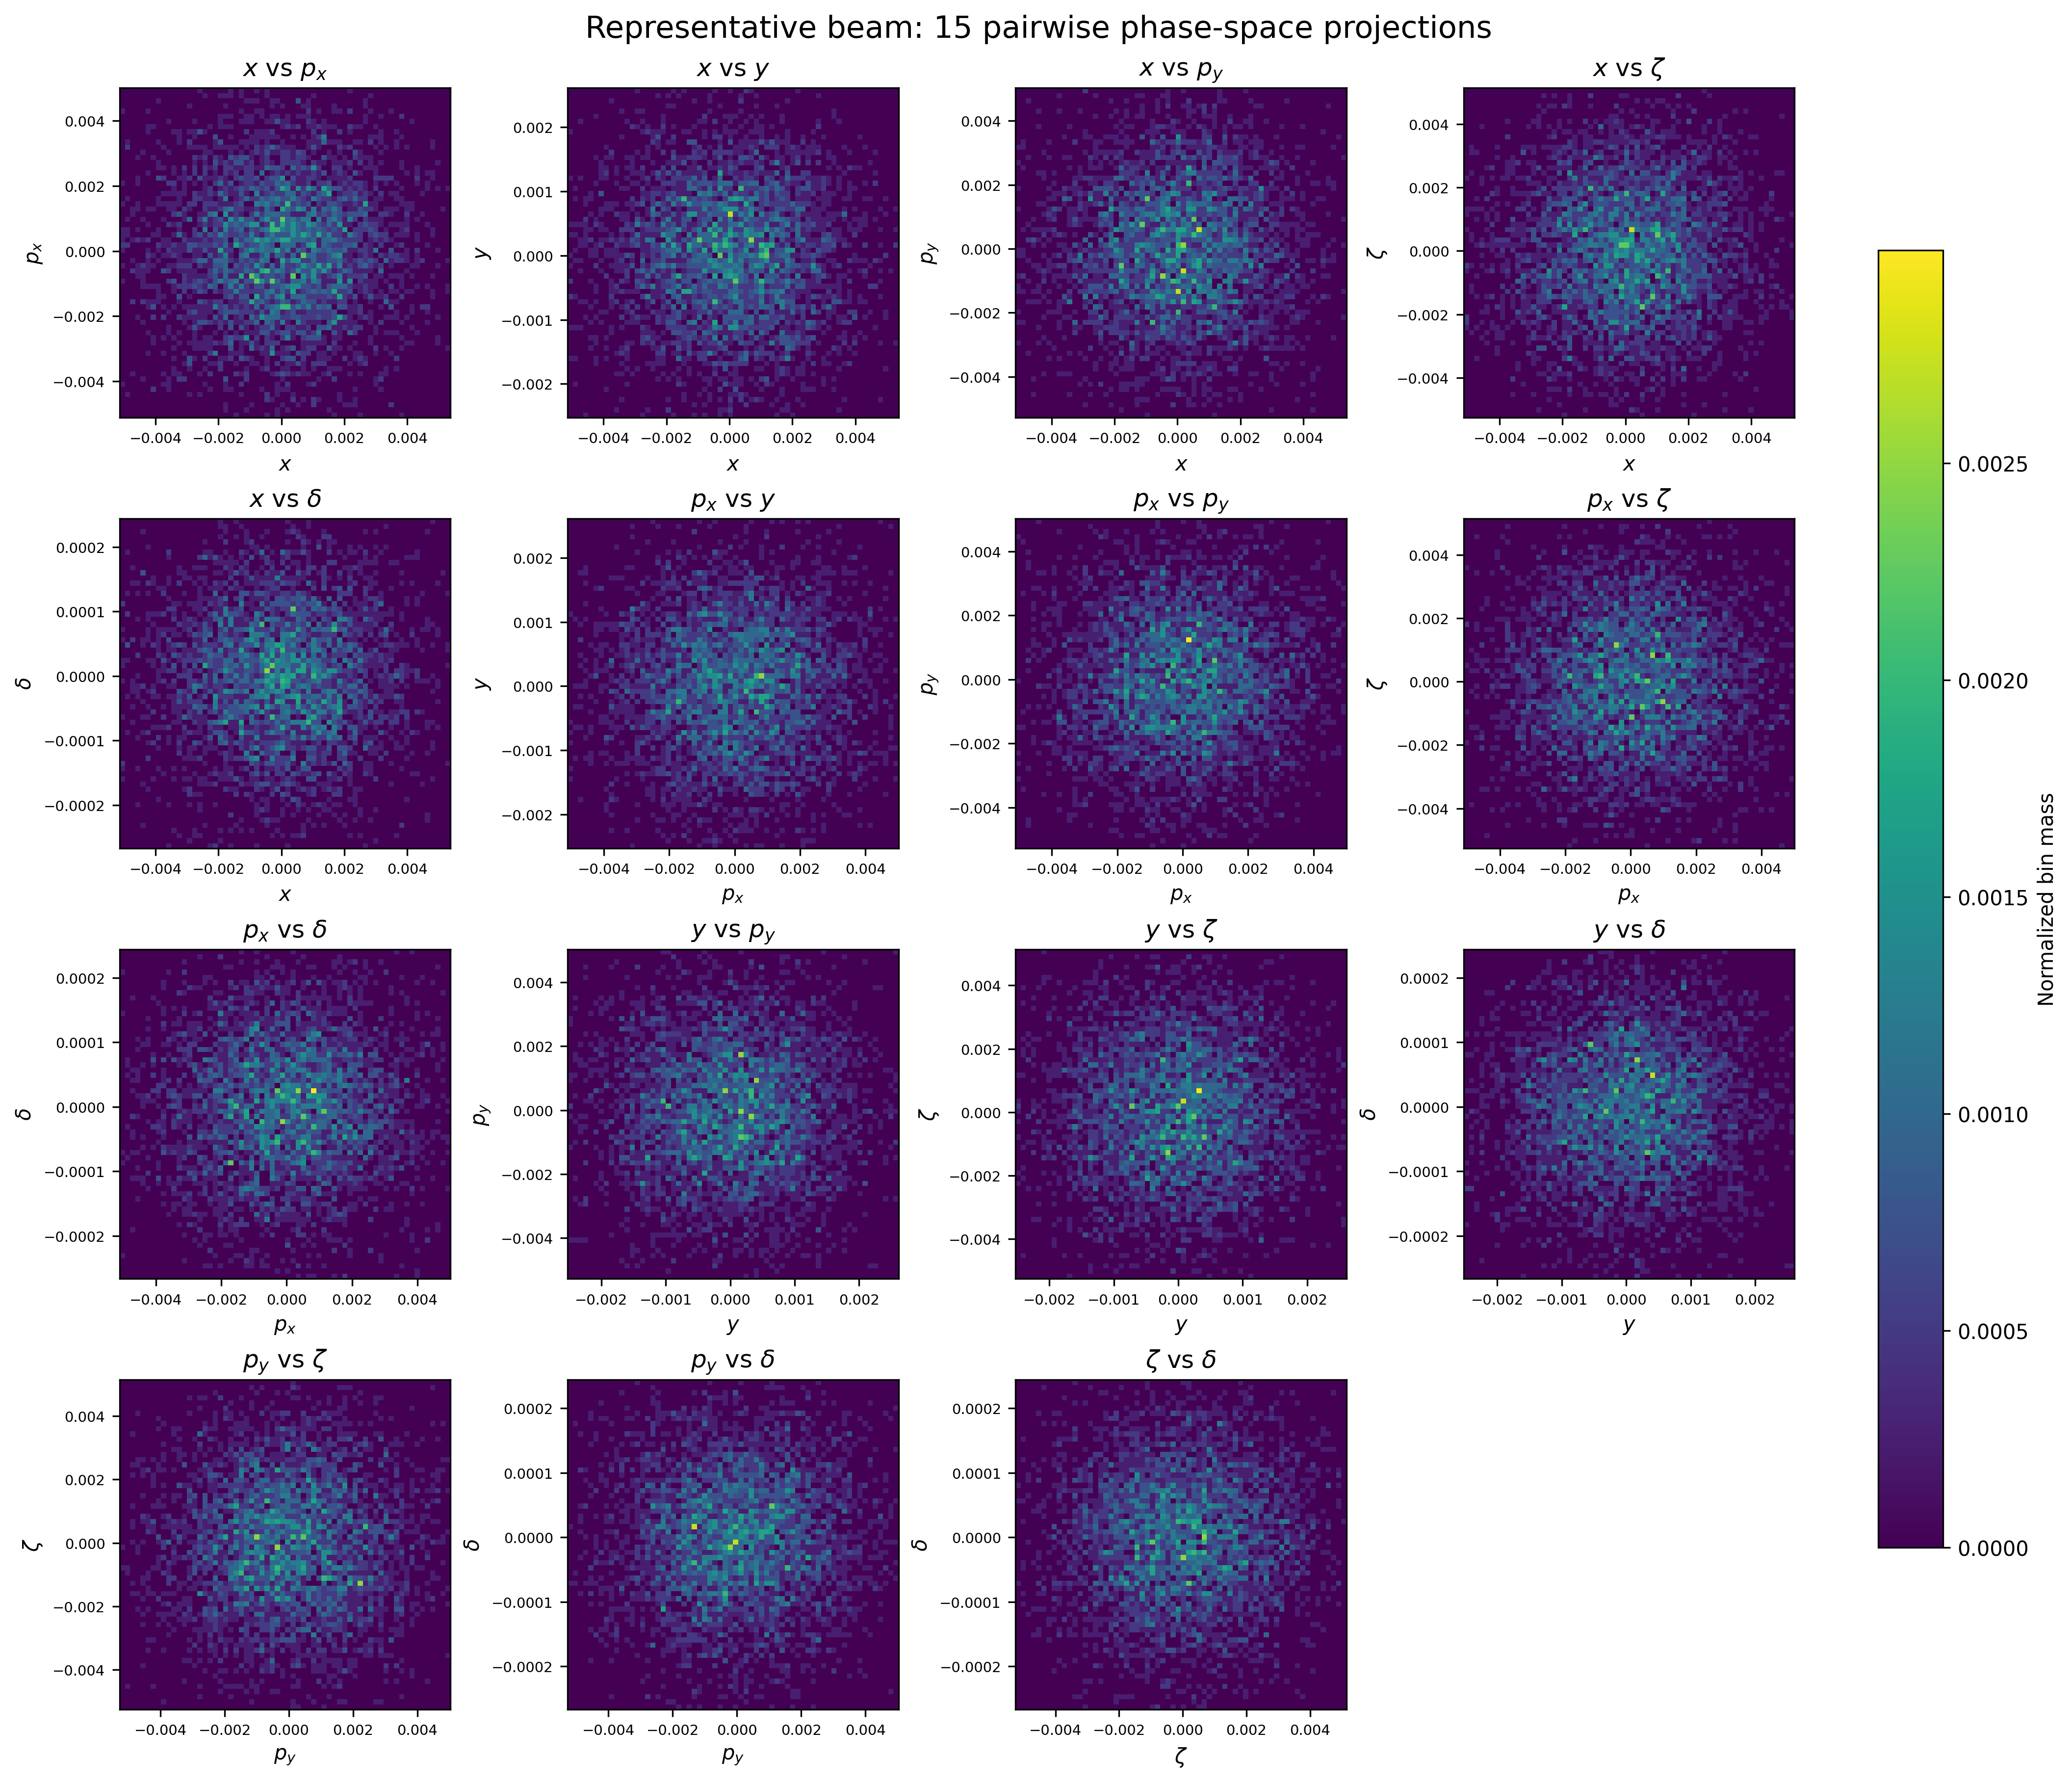
\includegraphics[width=\textwidth]{images/generated/dataset_representation.png}
    \caption{Representative beam state encoded through its fifteen pairwise two-dimensional phase-space marginals. The associated centroid and RMS vectors retain complementary information about physical position and extension. The figure represents a reduced description of a six-dimensional state, not a unique reconstruction of the complete joint density.}
    \label{fig:dataset_representation}
\end{figure}

% =============================================================================
